\section{Path Change Characterization}
\label{sec:char}

% FIGS 1--3 FROM SEC. 3
\begin{figure}[t]
%\begin{minipage}{0.33\textwidth}
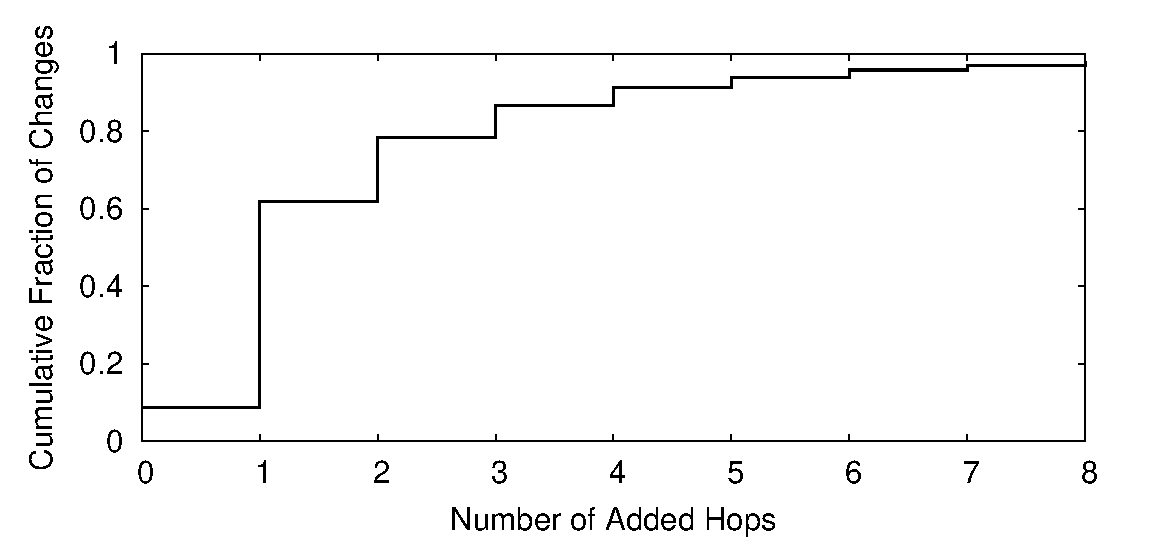
\includegraphics[width=\columnwidth]{figs/nadded.eps}
\caption{Number of hops added in path changes.}
\label{fig:char.nrouters}
%\end{minipage}
%\hfill

%\begin{minipage}{0.33\textwidth}
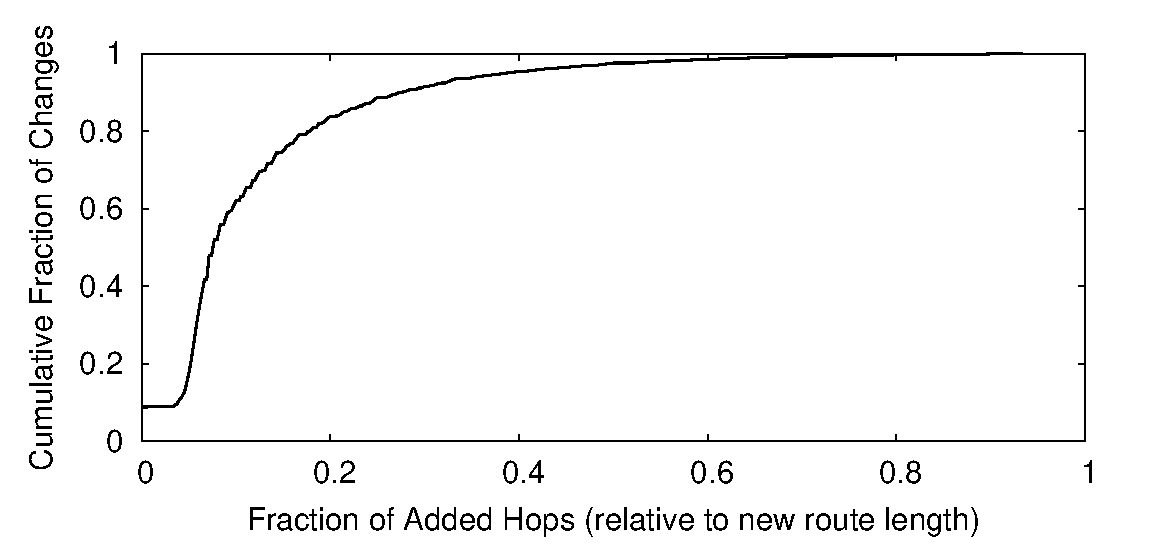
\includegraphics[width=\columnwidth]{figs/fracsadded.eps}
\caption{Fraction of hops added in path changes.}
\label{fig:char.fracs}
\end{figure}
%\end{minipage}
%\hfill
%\begin{minipage}{0.33\textwidth}
%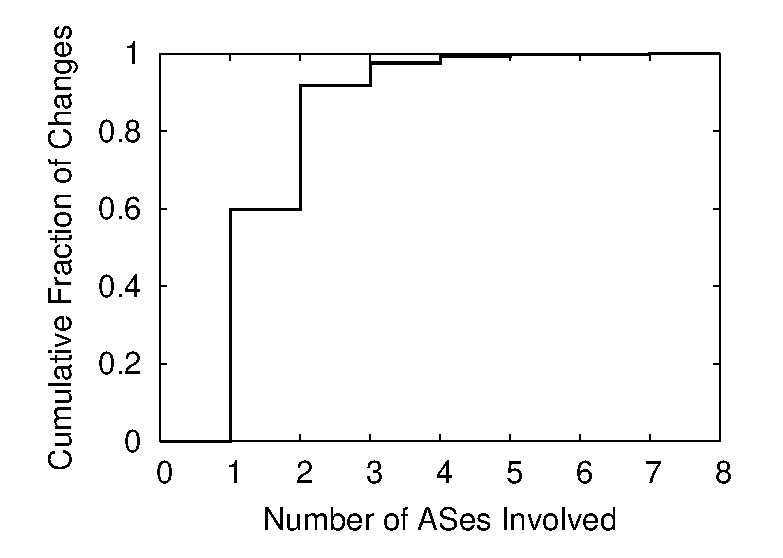
\includegraphics[width=1.05\textwidth]{figs/nasns.eps}
%\caption{Distribution of the number of ASes involved in path changes.}
%\label{fig:char.nasns}
%\end{minipage}

In this section we establish that most path changes involve few hops.
We deployed \dtrack{}~\cite{cunha11dtrack} (using complete remapping) to
track path changes from 72 PlanetLab nodes for one week starting March
4th, 2011.  Each monitor chose 1,000 destinations randomly from a list
of 34,820 reachable destinations.  We used a probing rate of 8 probes per
second, similar to the rate used by DIMES~\cite{shavitt09dimes}, and
observed 1,202,960  changes.  The observed paths traversed 7,315 ASes,
and 97\% of those with more than 50
customers~\cite{luckie13asrel}.\footnotemark{}

\footnotetext{Data sets publicly available at
www.dcc.ufmg.br/\url{~}cunha/datasets.}

%The number of hops added in a change is $h_c - h_d - 1$, assuming we know the previous route.

\figstr~\ref{fig:char.nrouters} shows the distribution of the number of
hops added by path changes, with one or more local change zones.  This
number represents the minimum number of hops we need to measure to
correctly map the new route.  We see that 78\% of changed paths add only
one or two hops, which is small compared to the median route length of
16 hops (not shown).  The most common type of path change (52\%)
replaces one hop with another.  We note that 9\% of changes only remove
hops from the old route. This may happen when probe filtering or
failures prevent hop measurement.


% \begin{figure}[t]
% \begin{center}
% 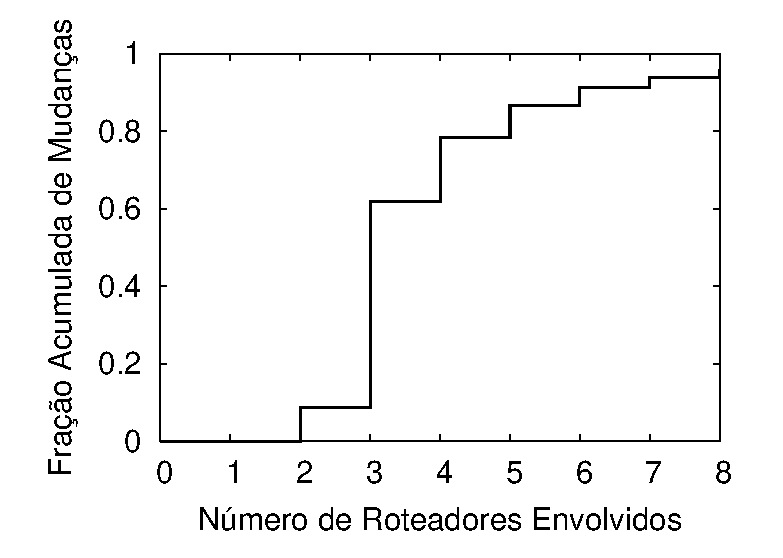
\includegraphics[width=0.8\columnwidth]{figs/nrouters.eps}
% \caption{Distribution of the number of hops involved in path changes.}
% \label{fig:char.nrouters}
% \vspace{-3mm}
% \end{center}
% \end{figure}

% \begin{figure}[t]
% \begin{center}
% 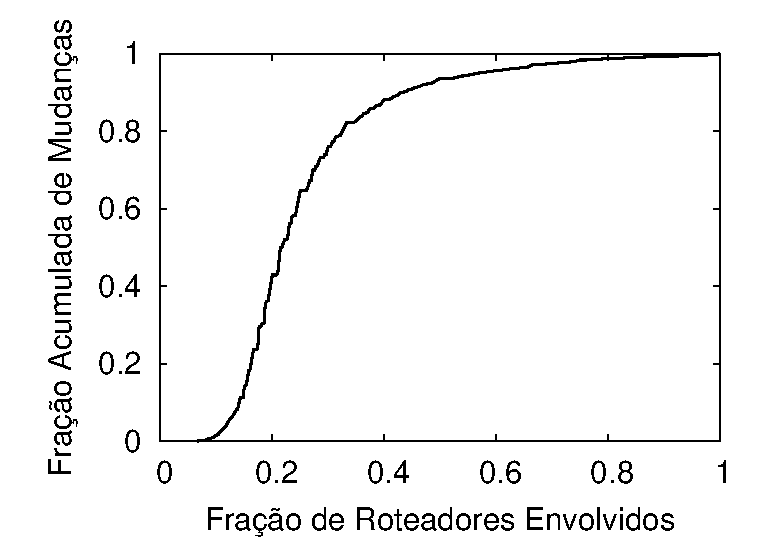
\includegraphics[width=0.8\columnwidth]{figs/fracs.eps}
% \caption{Distribution of the fraction of routers involved in path
% changes.}
% \label{fig:char.fracs}
% \vspace{-3mm}
% \end{center}
% \end{figure}

\figstr~\ref{fig:char.fracs} shows the distribution of the number of
added hops as a fraction of the (new) route length.  The curve is flat
before $x = 0.033 = 1/30$ as \dtrack{} only measures up to 30 hops in a
route (the default in Paris traceroute~\cite{veitch09balancer}).  In
80\% of cases less than 18\% of hops in the new route are new.  This
result shows the potential savings from local remapping compared to
complete remapping.

%We translate interface IP addresses measured by \dtrack{} to AS numbers
%combining IP-to-AS mapping databases from Team Cymru\footnotemark{} and
%iPlane~\cite{madhyastha06iplane}.  IP address that do not appear in any
%database are given their own fake AS number, resulting in
%overestimation.  \figstr~\ref{fig:char.nasns} shows the distribution of
%the number of ASes involved in a given path change.  We consider an AS
%to be involved if it contains any interface in a changed hop.  We find
%60\% of path changes are internal to a single AS, and only 7\% involve
%more than two.  The average number of hops inside each AS in a route is
%3.04.   These facts reinforce the finding that changes are local and
%involve few hops.  \ed{candidate for removal}

%\ed{christophe suggested looking at whether paths go back to the
%original routes after two changes.  will keep this in the queue.}

\footnotetext{Team Cymru, IP to ASN Mapping,
{http://www.team-cymru.org/}}
% Services/ip-to-asn.html}}

% \begin{figure}[t]
% \begin{center}
% 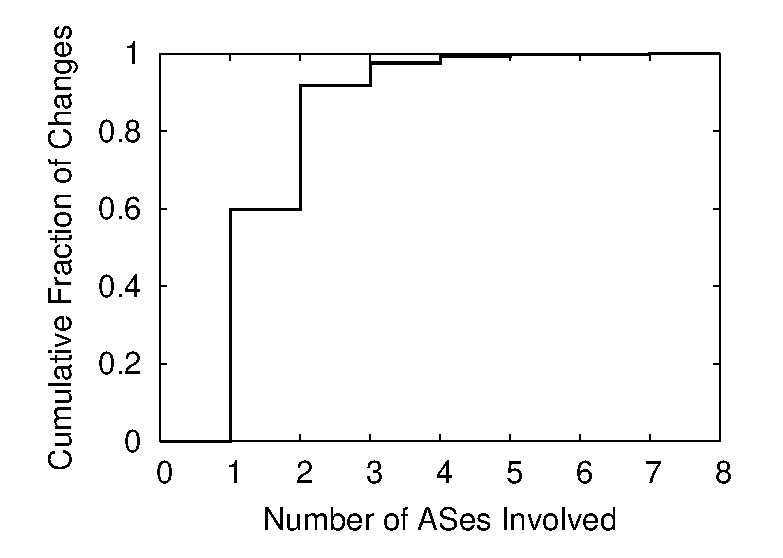
\includegraphics[width=0.8\columnwidth]{figs/nasns.eps}
% \caption{Distribution of the number of ASes involved in path changes.}
% \label{fig:char.nasns}
% \end{center}
% \end{figure}
